% lintrans - The linear transformation visualizer
% Copyright (C) 2021-2022 D. Dyson (DoctorDalek1963)

% This program is licensed under GNU GPLv3, available here:
% <https://www.gnu.org/licenses/gpl-3.0.html>

\documentclass[../development.tex]{subfiles}

\begin{document}

\subsubsection{Hiding the background and transformed grids\label{development:making-v0.2.2:hiding-the-background-and-transformed-grids}}

I spoke to my main stakeholder, who is the teacher that will be using \texttt{lintrans} when it's finished, and she said that the background grid and transformed grid can get a little bit in the way of the core action and make it harder to understand what's happening. Taking this feedback on board, I decided to add a display setting to toggle the background grid, and one to toggle the transformed grid.

I did the background grid first and then repeated everything for the transformed version of the grid as well. I am combining them here for brevity. The first step was of course to add a display setting for each of them. Then I had to add checkboxes for them in the display settings dialog, and then incorporate the settings into the actual drawing of the canvas.

%: d045057d568ac133b621ee9ca9daed361d570d7a
%: src/lintrans/gui/settings.py:14-27

%: d045057d568ac133b621ee9ca9daed361d570d7a
%: src/lintrans/gui/dialogs/settings.py:70,73,89-101,204,207-208,221,224-225 noscopes

%: d045057d568ac133b621ee9ca9daed361d570d7a
%: src/lintrans/gui/plots/widgets.py:60-63

%: d045057d568ac133b621ee9ca9daed361d570d7a
%: src/lintrans/gui/plots/classes.py:129-154

Then I added this change to the changelog.

%: d045057d568ac133b621ee9ca9daed361d570d7a
%: CHANGELOG.md:12-14 markdown!

\subsubsection{Hiding the basis vectors\label{development:making-v0.2.2:hiding-the-basis-vectors}}

While I was implementing new display settings, I decided to implement hiding basis vectors. This will give users the option of just seeing the grid get transformed. The process was exactly the same as before. Add the setting, add it to the dialog, use it when drawing.

%: 11ffbaf71f9fe29e1832a62f2b127aa3939e520d
%: src/lintrans/gui/settings.py:29-30

%: 11ffbaf71f9fe29e1832a62f2b127aa3939e520d
%: src/lintrans/gui/dialogs/settings.py:70,73,103-108,212,217,230,235 noscopes

%: 11ffbaf71f9fe29e1832a62f2b127aa3939e520d
%: src/lintrans/gui/plots/widgets.py:65-66

And then of course add it to the changelog.

%: 11ffbaf71f9fe29e1832a62f2b127aa3939e520d
%: CHANGELOG.md:12-14 markdown!

\subsubsection{Improving argument parsing\label{development:making-v0.2.2:improving-argument-parsing}}

Qt5 accepts arguments to its main method. I don't really know what these arguments can do, but it would be nice to be able to use them. I also want to be able to save sessions as files in the future, and it would be quite useful to open a session file by passing it as a command line argument. To make both of these easier, I decided to refactor my argument parsing.

Python has a built-in library called \pyinline{argparse}, which allows for more sophisticated argument parsing. One of the things \pyinline{argparse} can do is parse only some of the command line arguments with a method called \pyinline{parse_known_args()}\cite{argparse-parse-known-args}. I can then pass the unconsumed arguments on to Qt5. \texttt{\_\_main.py\_\_} now looks like this:

%: a688a14839caba2ee14f8551764b771ae803d935
%: src/lintrans/__main__.py

The \enquote{\pyinline{args[:1] + unparsed_args}} on line 71 means that we pass the name of the program first, and the rest of the unconsumed arguments after it.

And of course, I added it to the changelog, this time as a fix rather than an addition:

%: a688a14839caba2ee14f8551764b771ae803d935
%: CHANGELOG.md:16-18 markdown!

\subsubsection{Respecting display settings in the visual definition dialog\label{development:making-v0.2.2:respecting-display-settings-in-the-visual-definition-dialog}}

\texttt{DefineVisuallyWidget} is a subclass of \texttt{VisualizeTransformationWidget}. If it had its own instance attribute of type \pyinline{DisplaySettings}, then it could use its superclass's \pyinline{paintEvent()} method, and that would respect the display settings in the visual definition dialog.

%: 5850aa916b685992f31e58680267916927ed590d
%: src/lintrans/gui/plots/widgets.py:91-93

%: 5850aa916b685992f31e58680267916927ed590d
%: src/lintrans/gui/dialogs/define_new_matrix.py:169-180

Since the \texttt{DefineVisuallyDialog} now accepts display settings but the other definition dialogs don't, we need change the \pyinline{LintransMainWindow.dialog_define_matrix()} method to treat the visual definition dialog differently.

%: 5850aa916b685992f31e58680267916927ed590d
%: src/lintrans/gui/main_window.py:447-476

And, of course, I updated the changelog:

%: 5850aa916b685992f31e58680267916927ed590d
%: CHANGELOG.md:12,15 markdown!

\subsubsection{Changing the order in which things are drawn\label{development:making-v0.2.2:changing-the-order-in-which-things-are-drawn}}

Currently, \texttt{VisualizeTransformationWidget} draws the background, then the transformed grid, then the basis vectors, then the eigenlines and eigenvectors, then the determinant parallelogram and text. This means that the determinant parallelogram gets drawn on top of the basis vectors, which doesn't look very good. To fix this, we can simply re-order the drawing of different things. If we instead draw the transformed grid and basis vectors last, then they will appear on top of everything else, which should look significantly better.

I also renamed the \texttt{draw\_determinant\_text} display setting attribute to \texttt{show\_determinant\_value}.

Before:
%: e9da6737cbdb68e800c245bcc34e1c5c3824458a
%: src/lintrans/gui/plots/widgets.py:60-78

After:
%: acdf206a69d346dce67f74f2c54ff4c512c96229
%: src/lintrans/gui/plots/widgets.py:60-78

\begin{figure}[H]
	\hspace{0.03\linewidth}
	\begin{minipage}{0.45\linewidth}
		\begin{figure}[H]
			\centering
			\includegraphics[width=\linewidth]{development/5850aa916b685992f31e58680267916927ed590d/gui.png}
			\caption{Before re-ordering drawing commands}
			\label{fig:development:5850aa916b685992f31e58680267916927ed590d:gui.png}
		\end{figure}
	\end{minipage} \hfill
	\begin{minipage}{0.45\linewidth}
		\begin{figure}[H]
			\centering
			\includegraphics[width=\linewidth]{development/acdf206a69d346dce67f74f2c54ff4c512c96229/gui.png}
			\caption{After re-ordering drawing commands}
			\label{fig:development:acdf206a69d346dce67f74f2c54ff4c512c96229:gui.png}
		\end{figure}
	\end{minipage}
	\hspace{0.03\linewidth}
\end{figure}

\subsubsection{Improving online documentation with \textit{Read the Docs}\label{development:making-v0.2.2:improving-online-documentation-with-read-the-docs}}

So far, I've been building my documentation automatically using a tool called \texttt{Sphinx}\cite{sphinx}. I've been using it to scan through my source code, extract all the docstrings\cite{pep257-docstring-conventions}, and compile a HTML version of the source code documentation. I then publish this documentation to GitHub Pages\cite{github-pages-docs}, and all that happens automatically along with the unit tests whenever I push my changes to GitHub.

However, this system can't track changes in documentation over time. There's a popular website for hosting open source documentation, especially for Python packages, called \textit{Read the Docs}\cite{readthedocs-homepage}. It would be nice to host my documentation on there, since it would provide a standard build for the docs, and would allow me to keep track of documentation for different versions over time. I read through their tutorial and followed along with it, and then I could use Read the Docs for \texttt{lintrans}.

%: a7a8aa09148f4acf8591547d6d8b9cd8b8d52905
%: .readthedocs.yaml language=yaml

This file governs the build pipeline for the documentation. It defines how the docs will be built on the remote machine. It basically just installs all the dependencies and \texttt{lintrans} itself in a virtual environment, generates the object inventory for \texttt{intersphinx} (see \S\ref{development:preparing-for-v0.2.1:linking-in-documentation}), builds the internal import graph (see \S\ref{development:fumbling-with-semver:adding-a-graph-of-internal-imports}), and makes sure that lintrans can be installed successfully in the virtual environment. The string \enquote{\mintinline{sh}{$(pwd | sed "s/checkouts\(\/[^/]\+\)\/docs\$/envs\1/")/bin/python}} appears frequently. This string finds the version of Python that will be used for building the actual documentation at the end of the pipeline. \texttt{lintrans} has some issues with circular imports, which means that it can only be installed in editable mode\footnote{Editable mode is an option that you can choose when installing a package with \texttt{pip}\cite{pip-install-editable}. Instead of copying the source code to the installation directory like normal, it creates a link to the source code from the installation directory - basically a symlink in Linux. This means that if you change the source code, the installed version gets updated instantly, which is obviously very useful for fast, iterative development. It also has some strange effects with import order and resolution. Importing packages and modules is very complicated in Python\cite{david-beazley-python-modules}, and I repeatedly failed to get \texttt{lintrans} to be installable without editable mode, so I had to resort to just using this bodge on Read the Docs instead.}. This means that I have to bodge the build system to install \texttt{lintrans} properly.

Additionally, having a build system like this means that builds should be repeatable, which means I should pin the exact versions of all my dependencies, to avoid any breaking changes in the future.

%: 152f9e59b5b4e22607cf2b687c85c70708054579
%: requirements.txt language="lexers.py:CommentedTextLexer -x"

%: 152f9e59b5b4e22607cf2b687c85c70708054579
%: dev_requirements.txt language="lexers.py:CommentedTextLexer -x"

%: 152f9e59b5b4e22607cf2b687c85c70708054579
%: docs/docs_requirements.txt language="lexers.py:CommentedTextLexer -x"

Now that I was using Read the Docs, I could remove the old GitHub Actions workflow to compile the documentation.

\end{document}
